\documentclass[UTF8,fontset=macnew,xcolor=table]{ctexbeamer}
\usepackage{indentfirst}
\usepackage{color}
\usepackage{xcolor}
\usepackage{enumerate}
\usepackage{listings}
\usepackage{multimedia}
\usepackage{multicol}

\usefonttheme[onlymath]{serif}

\setlength{\parindent}{2em}
\usetheme{CambridgeUS}
\useoutertheme{smoothbars}
\setbeamercolor{normal text}{bg=black!10}
\definecolor{ustcblue}{cmyk}{1,0.8,0,0}

\definecolor{uibred}  {HTML}{db3f3d}
\definecolor{uibblue} {HTML}{4ea0b7}
\definecolor{uibgreen}{HTML}{789a5b}
\definecolor{uibgray} {HTML}{d0cac2}
\definecolor{uiblink} {HTML}{00769E}
\setbeamertemplate{enumerate items}[default]
\setbeamercolor{block body} {bg = uibgray}
\setbeamercolor{block title}{fg = white,bg = uibred}

\renewcommand\lstlistingname{代码}

% \lstset{
%     basicstyle          =   \sffamily,          % 基本代码风格
%     keywordstyle        =   \bfseries,          % 关键字风格
%     commentstyle        =   \rmfamily\itshape,  % 注释的风格,斜体
%     stringstyle         =   \ttfamily,  % 字符串风格
%     flexiblecolumns,                % 别问为什么,加上这个
%     numbers             =   none,   % 行号的位置在左边
%     showspaces          =   false,  % 是否显示空格,显示了有点乱,所以不现实了
%     numberstyle         =   \zihao{-5}\ttfamily,    % 行号的样式,小五号,tt等宽字体
%     showstringspaces    =   false,
%     captionpos          =   t,      % 这段代码的名字所呈现的位置,t指的是top上面
%     frame               =   lrtb,   % 显示边框
%     captionpos          =   b       % caption的位置(填t在上,填b在底部)
% }

\definecolor{mygreen}{rgb}{0,0.6,0}
\definecolor{mygray}{rgb}{0.5,0.5,0.5}
\definecolor{mymauve}{rgb}{0.58,0,0.82}

\lstdefinestyle{Text}{
    language        =   Python, % 语言选Python
    basicstyle      =   \zihao{-5}\ttfamily,
    numberstyle     =   \zihao{-5}\ttfamily,
    keywordstyle    =   \color{black},
    keywordstyle    =   [2] \color{black},
    stringstyle     =   \color{black},
    commentstyle    =   \color{black}\ttfamily,
    breaklines      =   true,   % 自动换行,建议不要写太长的行
    columns         =   fixed,  % 如果不加这一句,字间距就不固定,很丑,必须加
    basewidth       =   0.5em,
}

\lstset{ %
backgroundcolor=\color{white},      % choose the background color
basicstyle=\footnotesize\ttfamily,  % size of fonts used for the code
columns=fullflexible,
tabsize=4,
breaklines=true,               % automatic line breaking only at whitespace
captionpos=t,                  % sets the caption-position to bottom
commentstyle=\color{mygreen},  % comment style
escapeinside={\%*}{*)},        % if you want to add LaTeX within your code
keywordstyle=\color{blue},     % keyword style
stringstyle=\color{mymauve}\ttfamily,  % string literal style
frame=lrtb,
rulesepcolor=\color{red!20!green!20!blue!20},
% identifierstyle=\color{red},
}


\begin{document}
\title[结题报告——sBPF]{\huge 结题报告}
%\subtitle[副题简称]{论文副题}
\author[中国科学技术大学]{陈思睿 \and 梁恒宇 \and 吕泓涛 \and 汤力宇}
\institute[USTC]{中国科学技术大学}
\date[\today]{\today}
\logo{\textcolor{ustcblue}{\includegraphics[scale=0.25]{ustc_logo_side.pdf}}}
\begin{frame}
    \titlepage
\end{frame}

\section{项目概括}
\begin{frame}{sBPF——介于用户态与内核态之间的轻量级沙盒}
    \begin{columns}
        \begin{column}{0.75\textwidth}
            \begin{itemize}
                \item 特权级别——linux主要分为用户态与内核态
                \item 用户态进程——内核态进程
                \item 用户态内存——内核态内存
                
                \item \textbf{\Large 复杂的中断、调度、拷贝机制!!}\\
                给沙盒的实现带来了困难
                
            \end{itemize}
        \end{column}

        \begin{column}{0.25\textwidth}
            \begin{figure}[H]
                \centering
                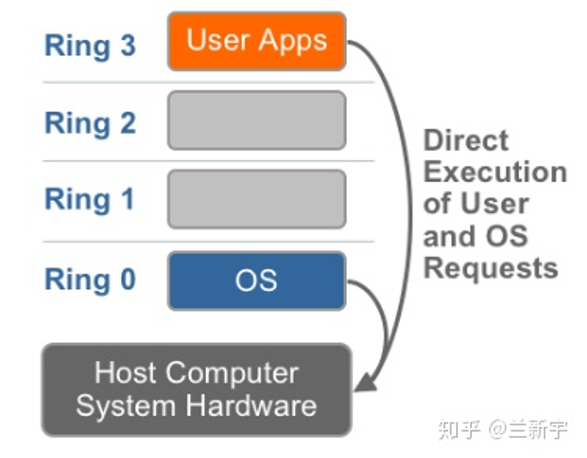
\includegraphics[width=\columnwidth]{pic1.png}
            \end{figure}
        \end{column}
    \end{columns}
\end{frame}

\section{背景知识}
\begin{frame}{内核态沙盒工具}
    \begin{columns}
        \begin{column}{0.5\textwidth}
            \begin{itemize}
                \item Seccomp
                \item Namespace
                \item Cgroup
                
                \item 灵活性差 
                \item 只能实现最基本的功能
                \item 大部分无法独立工作,需要用户态程序协作
            \end{itemize}
        \end{column}

        \begin{column}{0.5\textwidth}
            \begin{figure}[H]
                \centering
                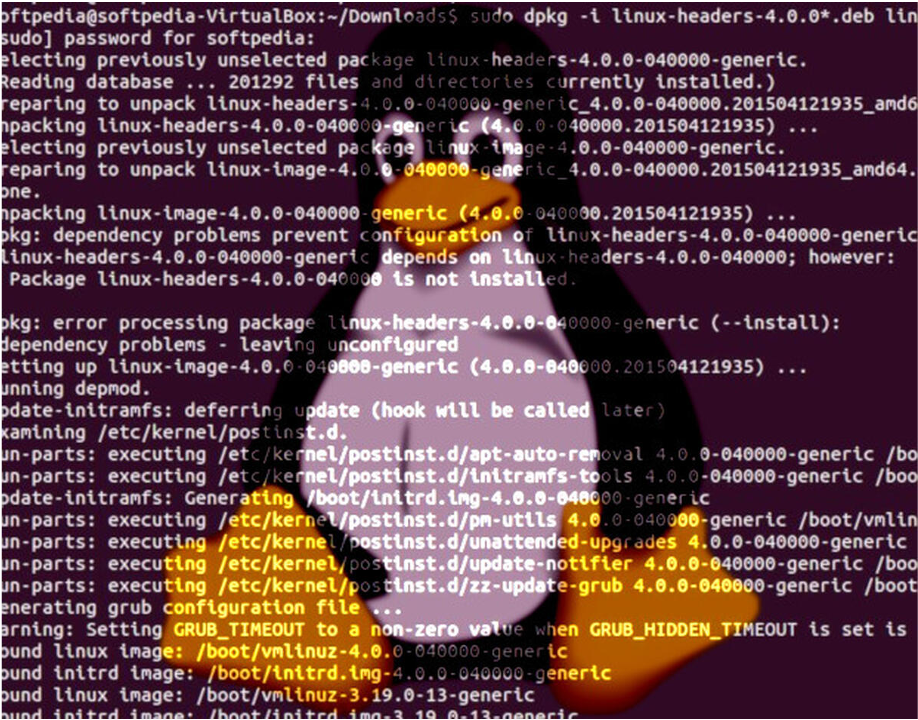
\includegraphics[width=\columnwidth]{pic2.png}
            \end{figure}
        \end{column}
    \end{columns}
\end{frame}

\begin{frame}{用户态沙盒}
    \begin{columns}
        \begin{column}{0.5\textwidth}
            \begin{itemize}
                \item gVisor
                \item Docker
                
                
                \item 需要将数据流与控制流在内核态与用户态间多次中转
                \item 性能损失
                \item 面临程序被篡改的安全性问题
            \end{itemize}
        \end{column}

        \begin{column}{0.5\textwidth}
            \begin{figure}[H]
                \centering
                
\includegraphics[width=\columnwidth]{pic3.png}
            \end{figure}
        \end{column}
    \end{columns}
\end{frame}

\section{项目框架}
\begin{frame}{我们的解决方案:半用户态半内核态沙盒}
    \begin{columns}
        \begin{column}{0.5\textwidth}
            \begin{block}{用户:}
            \begin{itemize}
                \item 编写沙盒处理程序
                \item 直接注入到内核中
                \item 得到一个高度自由的沙盒程序
            \end{itemize}
            \end{block}
        \end{column}

        \begin{column}{0.5\textwidth}
            \begin{block}{内核:}
                \begin{itemize}
                    \item 提供沙盒处理程序挂在点
                    \item 提供沙盒处理程序调用机制
                    \item 在内核中直接完成沙盒执行
                \end{itemize}
                \end{block}
        \end{column}
    \end{columns}
\end{frame}

\begin{frame}{机制与策略相分离}

    \begin{itemize}
        \item 少量内核代码定义写死的沙盒机制
        大量通用代码提供灵活的沙盒策略,实现不同的行为模式\\
        
        \item 我们做到了:
        \item 使用最少的内核代码,只起调用功能(20行内)
        \item 提供丰富多样的沙盒行为模块代码(3.5套不同的行为模式)
        \item 便于测试、升级、实现各种灵活的功能
    \end{itemize}
    
\end{frame}

\begin{frame}{在安全问题上我们的思考}
    \begin{columns}
        \begin{column}{0.8\textwidth}
            \begin{itemize}
                \item 数据安全是日常生活中最重要的计算机安全问题
                \item 企业机密
                \item 个人隐私
                \item 重要账密
                \item 数据绑架
            \end{itemize}
        \end{column}

        \begin{column}{0.2\textwidth}
            \begin{figure}[H]
                \centering
                
\includegraphics[width=\columnwidth]{pic4.png}
            \end{figure}
        \end{column}
    \end{columns}
\end{frame}

\begin{frame}{我们的选择与妥协}

    \begin{itemize}
        \item 重点进行文件保护
        \item 其余方面通过现有的内核沙盒工具进行防护\\
        
        \item 减轻工作量
        \item 设计方法论的验证
    \end{itemize}
    
\end{frame}

\begin{frame}{介入方法}
    \begin{columns}
        \begin{column}{0.7\textwidth}
            \begin{itemize}
                \item 介入系统调用
                \item 在系统调用的进入位置添加静态插桩点,直接获取上下文参数,介入运行流程,交给内核态处理程序运行\\
                
                \item 对比传统沙盒:
                \item 使用ptrace等内核工具
                \item 动态插桩点对内核版本不稳定
                \item 用户态处理程序,上下文切换
            \end{itemize}
        \end{column}

        \begin{column}{0.3\textwidth}
            \begin{figure}[H]
                \centering
                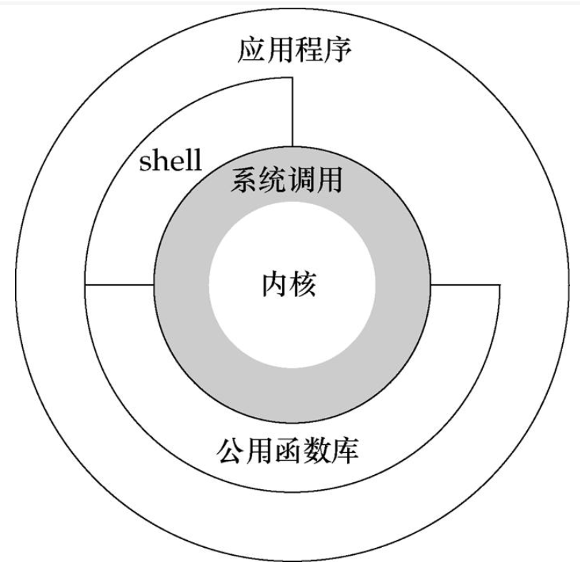
\includegraphics[width=\columnwidth]{pic5.png}
            \end{figure}
        \end{column}
    \end{columns}
\end{frame}

\begin{frame}{沙盒处理程序的工作方式}

    \begin{itemize}
        \item 直接利用钩子函数实现调用,由于运行在内核态,可以简单直接的使用内核api来进行编程\\

        \item 对比传统沙盒:
        \item 复杂的回调机制触发运行
        \item 依赖系统调用来维持自身运行
        \item 返回值依赖内核的复杂传回机制传回
    \end{itemize}
    
\end{frame}

\begin{frame}{管理程序工作方式}

    \begin{itemize}
        \item 简单的调用被监测的程序
        \item 简单的诸如沙盒行为代码
        \item 通过成熟的api调用cgourp功能实现资源保护
        \item 整体结构简单\\
        
        \item 对比传统沙盒的工作方式
        \item 需要管理大量的数据结构和程序段,体量庞大,难以编写和调试
    \end{itemize}
    
\end{frame}

\begin{frame}{从代码角度上来说}

    \begin{itemize}
        \item {\ttfamily Loader} : 用户态管理程序

        \item {\ttfamily sBPF\_xxx} : 注入内核的沙盒行为代码 
        
        \item {\ttfamily test\_programme} : 被隔离程序
    \end{itemize}
    
\end{frame}

\begin{frame}{实现的文件保护行为模式}

    \begin{itemize}
        \item {\ttfamily sBPF\_redir} 简单的目录重映射模式 
        完整的虚拟目录系统
        映射所有读写操作
        
        \item {\ttfamily sBPF\_cow} 对写操作进行备份的copy on write模式
        允许读原始文件系统
        写入文件时,将文件复制到沙盒文件目录
        对修改过的文件的读写操作都映射到沙盒目录
        
        \item {\ttfamily sBPF\_permission} 自定义文件访问权限模式
    \end{itemize}
    
\end{frame}

\section{功能演示}
\begin{frame}{行为演示}

\begin{figure}[H]
    \centering
    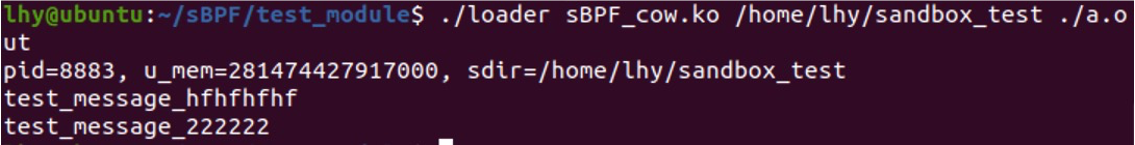
\includegraphics[width=0.55\columnwidth]{pic6.png}
    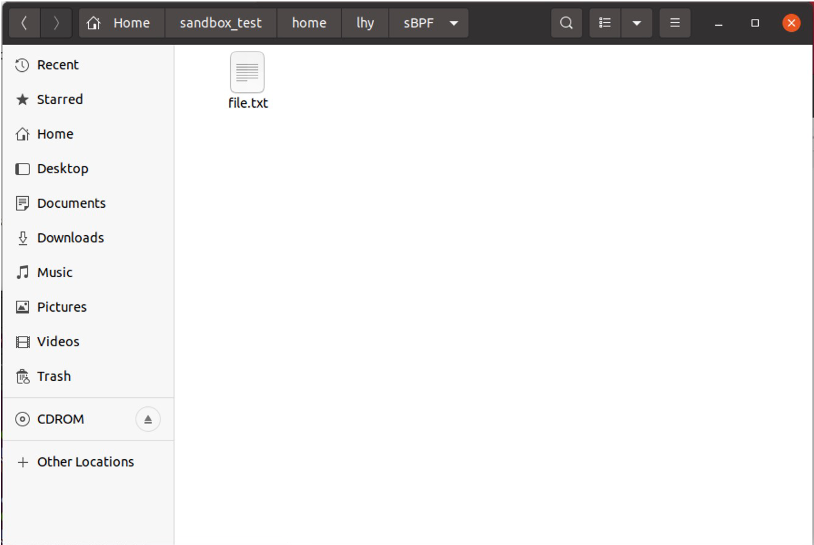
\includegraphics[width=0.5\columnwidth]{pic7.png}
    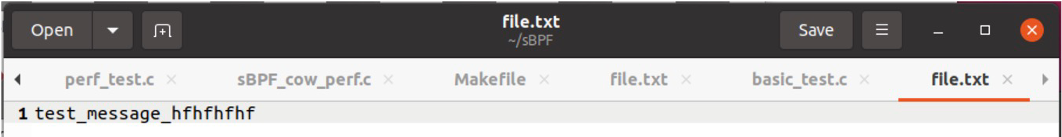
\includegraphics[width=0.55\columnwidth]{pic8.png}
    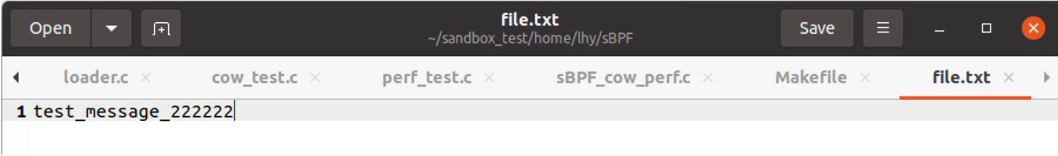
\includegraphics[width=0.55\columnwidth]{pic9.png}
\end{figure}

\end{frame}

\section{性能测试}
\begin{frame}{性能测试}

\begin{figure}[H]
    \centering
    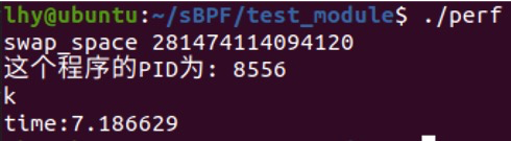
\includegraphics[width=0.4\columnwidth]{pic11.png}
    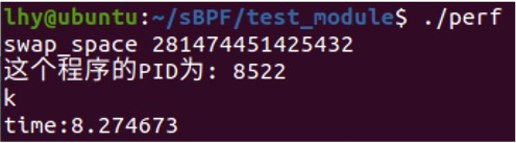
\includegraphics[width=0.4\columnwidth]{pic12.png}
    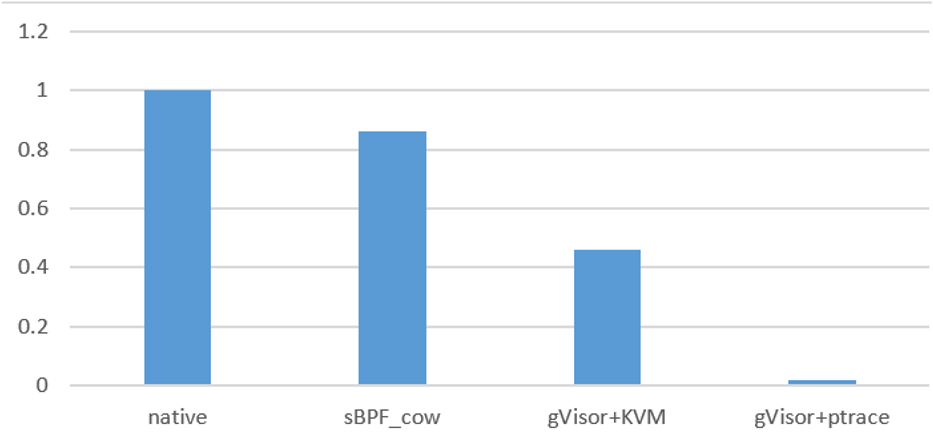
\includegraphics[width=0.8\columnwidth]{pic13.png}
\end{figure}
    
\end{frame}

\section{Q\&A}
\begin{frame}{Q\&A}
    
\end{frame}

\end{document}